\begin{activity} \label{A:3.1.2}  Suppose that $g$ is a function whose second derivative, $g''$, is given by the following graph.
\begin{figure}[h]
\hfil
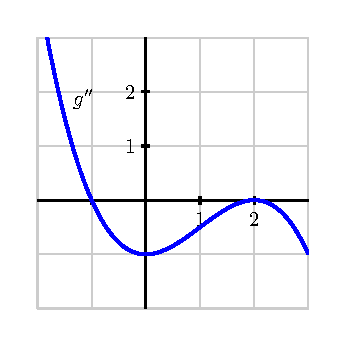
\includegraphics{figures/3_1_Act2.eps} 
\hfil
\caption{The graph of $y = g''(x)$.} \label{F:3.1.Act2}
\end{figure}
\ba 
  \item Find all points of inflection of $g$. 
  \item Fully describe the concavity of $g$ by making an appropriate sign chart.  
  \item Suppose you are given that $g'(-1.67857351) = 0$.  Is there is a local maximum, local minimum, or neither (for the function $g$) at this critical value of $g$, or is it impossible to say?  Why?
  \item Assuming that $g''(x)$ is a polynomial (and that all important behavior of $g''$ is seen in the graph above, what degree polynomial do you think $g(x)$ is?  Why?
\ea
\end{activity}
\begin{smallhint}
\ba 
  \item What must be true of $g''(x)$ at a point of inflection?
  \item Use the given graph to decide where $g''$ is positive and negative.
  \item What does the second derivative test say?
  \item Can you guess a formula for $g''(x)$ based on its graph?
\ea
\end{smallhint}
\begin{bighint}
\ba 
  \item At what points on the given graph does $g''(x)$ change sign?
  \item From the given graph, where is $g''(x) > 0$?  $g''(x) < 0$?
  \item What does the second derivative test say?  What is $g''(-1.67857351)$?
  \item Can you guess a formula for $g''(x)$ based on its graph?  Note that $g''$ appears to have a repeated root at $x = 2$.
\ea
\end{bighint}
\begin{activitySolution}
\ba 
  \item Based on the given graph of $g''$, the only point at which $g''$ changes sign is $x = -1$, and hence this is an inflection point of $g$. 
  \item Note that $g''(x) > 0$ for $x < -1$, $g''(x) < 0$ for $-1 < x < 2$, and $g''(x) < 0$ for $x > 2$.  This tells us that $g$ is concave up for $x < -1$, concave down for $-1 < x < 2$, and concave down for $x > 2$.
  \item Given that $g'(-1.67857351) = 0$, we know that $g$ has a horizontal tangent line at this critical value.  In addition, from the given graph of $g''$, we see that $g''( -1.67857351) > 0$ and observe that $g$ is concave up at $x$-values near $-1.67857351$.  By the second derivative test, $g$ has a local minimum at $x = -1.67857351$.
  \item From the given graph, since $g''$ has a simple zero at $x = -1$ and a repeated zero at $x = 2$, it appears that $g''$ is a degree 3 polynomial.  If so, then $g'$ is a degree 4 polynomial, and $g$ is a degree 5 polynomial.
\ea
\end{activitySolution}
\aftera